\begin{equation} \label{eq_hofelvetel}
\dot Q_{fel} = c ~ \dot{m} ~ \Delta t
\end{equation}


\begin{equation} \label{eq_holeadas2}
\begin{aligned}
\dot Q_{le} = k_e ~ A_e ~ \left( \frac{t_s+t_r}{2}-t_i\right) = k_e ~ A_e ~ \left( \frac{t_s+(t_s-\Delta t)}{2}-t_i-t_{drop}\right)
\end{aligned}
\end{equation}

Ahol felhasználtuk azt is, hogy $t_r = t_s-\Delta t$, majd $\Delta t$ helyére beírhatjuk a (\ref{eq_hofelvetel})  átrendezett alakját:
\begin{equation} \label{eq_hofelvetel2}
~~\Delta t = \frac{\dot Q_{fel}}{c ~ \dot{m}}
\end{equation}

Beírva (\ref{eq_holeadas2})-ba (\ref{eq_hofelvetel2})-t:

A \ref{f}. figure

\begin{figure}
	\centering
	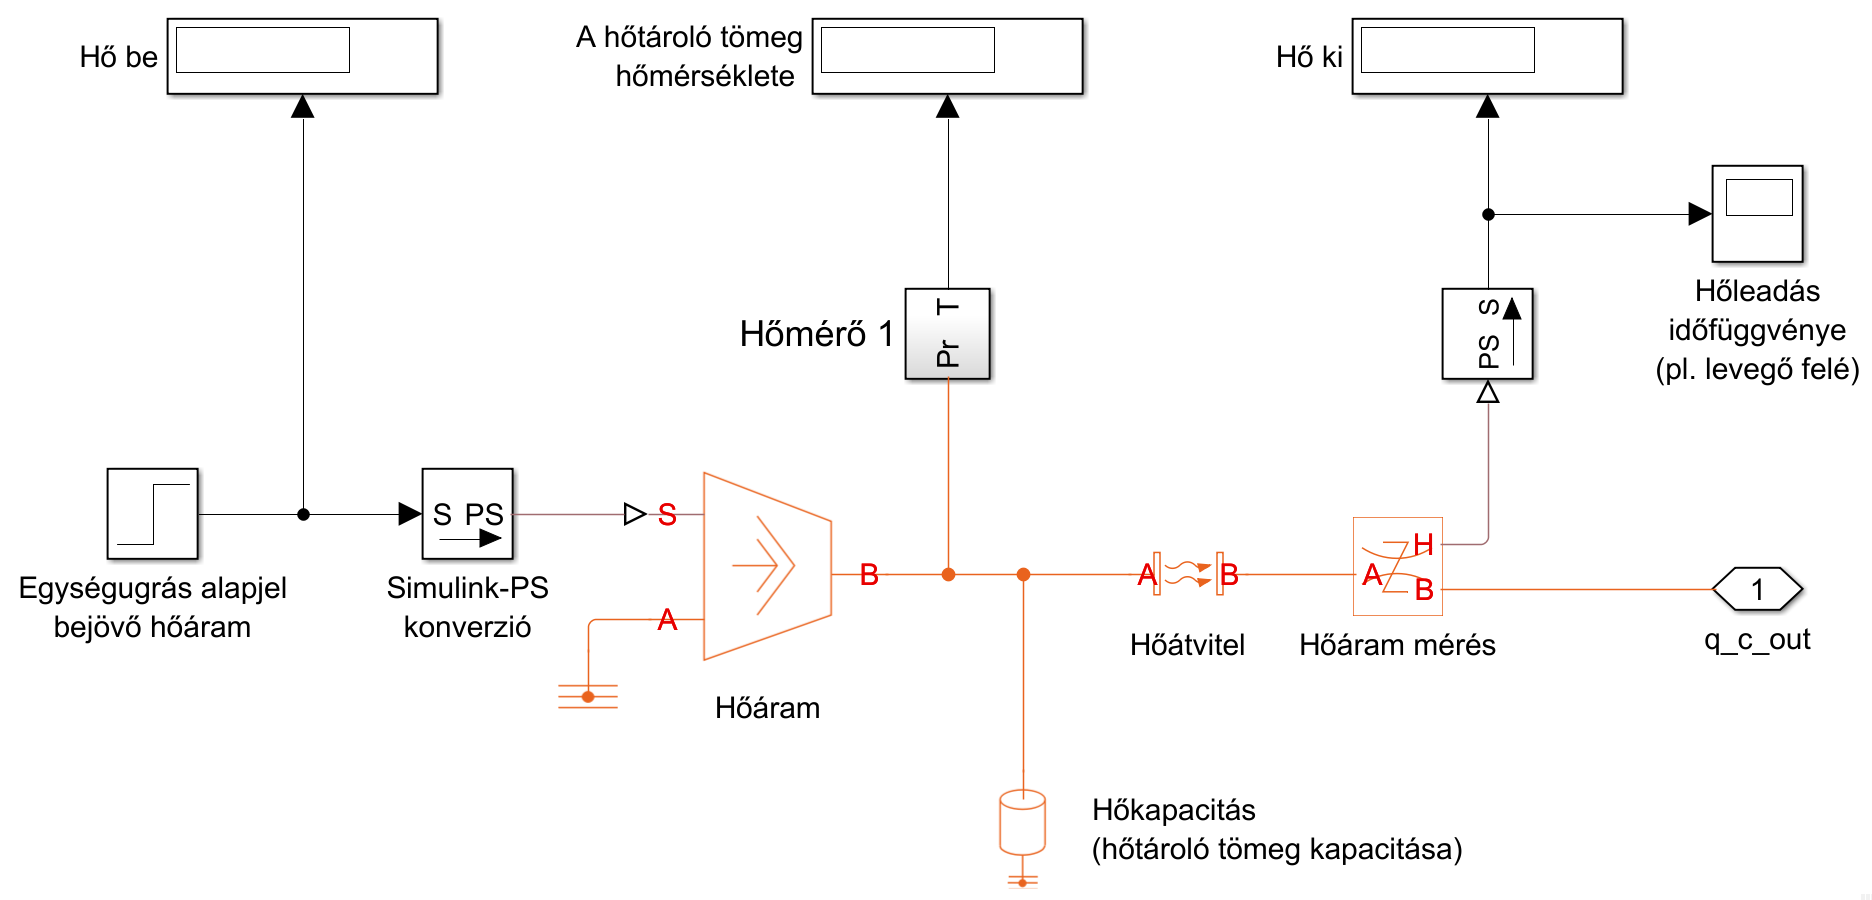
\includegraphics[width=\textwidth]{figures/SimscapeGeneral}
	\caption{Simscape termikus blokkok a Simulinkben}
	\label{f}
\end{figure}

A \ref{f}. figure